\documentclass[10pt,twocolumn,letterpaper]{article}

\usepackage{cvpr}
\usepackage{times}
\usepackage{epsfig}
\usepackage{graphicx}
\usepackage{amsmath}
\usepackage{amssymb}
\usepackage[utf8]{inputenc}
\usepackage{verbatim}
\usepackage[pagebackref=true,breaklinks=true,letterpaper=true,colorlinks,bookmarks=false]{hyperref}

\graphicspath{{images/}}

toto powa

% \cvprfinalcopy % *** Uncomment this line for the final submission

\def\cvprPaperID{1120} % *** Enter the CVPR Paper ID here
\def\httilde{\mbox{\tt\raisebox{-.5ex}{\symbol{126}}}}

% Pages are numbered in submission mode, and unnumbered in camera-ready
\ifcvprfinal\pagestyle{empty}\fi
\begin{document}

%%%%%%%%% TITLE
\title{Yeah}

\author{Placeholder Author}

\maketitle
% \thispagestyle{empty}
%\includegraphics[width=.44\linewidth]{}




\section{Introduction}

Birds rock.

%-------------------------------------------------------------------------
\subsection{Language}

All manuscripts must be in English.


\includegraphics[width=2.5cm]{a_bird.png}
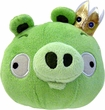
\includegraphics[width=3cm]{a_pig.png}

\includegraphics[width=2cm]{a_bird.png}

one

two

\subsection{Dual submission}

three

By submitting a manuscript to ICCV, the authors assert that it has not been
previously published in substantially similar form. Furthermore, no paper
which contains significant overlap with the contributions of this paper
either has been or will be submitted during the
(2)~argue in the body of your paper why your CVPR paper is non-trivially
different from these concurrent submissions, and (3)~include anonymized
versions of those papers in the supplemental material.

\subsection{Paper length}
CVPR papers may be between 6 pages and 8 pages, with a \$100 per page added
fee.  Overlength papers will simply not be reviewed.  This includes papers
where the margins and formatting are deemed to have been significantly
altered from those laid down by this style guide.  Note that this
\LaTeX\ guide already sets figure captions and references in a smaller font.
The reason such papers will not be reviewed is that there is no provision for
supervised revisions of manuscripts.  The reviewing process cannot determine
the suitability of the paper for presentation in eight pages if it is
reviewed in eleven.  If you submit 8 for review expect to pay the added page
charges for them. 

\end{document}
